\documentclass[]{article}
\usepackage{lmodern}
\usepackage{amssymb,amsmath}
\usepackage{ifxetex,ifluatex}
\usepackage{fixltx2e} % provides \textsubscript
\ifnum 0\ifxetex 1\fi\ifluatex 1\fi=0 % if pdftex
  \usepackage[T1]{fontenc}
  \usepackage[utf8]{inputenc}
\else % if luatex or xelatex
  \ifxetex
    \usepackage{mathspec}
    \usepackage{xltxtra,xunicode}
  \else
    \usepackage{fontspec}
  \fi
  \defaultfontfeatures{Mapping=tex-text,Scale=MatchLowercase}
  \newcommand{\euro}{€}
\fi
% use upquote if available, for straight quotes in verbatim environments
\IfFileExists{upquote.sty}{\usepackage{upquote}}{}
% use microtype if available
\IfFileExists{microtype.sty}{%
\usepackage{microtype}
\UseMicrotypeSet[protrusion]{basicmath} % disable protrusion for tt fonts
}{}
\usepackage[margin=1in]{geometry}
\ifxetex
  \usepackage[setpagesize=false, % page size defined by xetex
              unicode=false, % unicode breaks when used with xetex
              xetex]{hyperref}
\else
  \usepackage[unicode=true]{hyperref}
\fi
\usepackage[usenames,dvipsnames]{color}
\hypersetup{breaklinks=true,
            bookmarks=true,
            pdfauthor={Carlos T. Estrada Arzamendi},
            pdftitle={IO2 PS2: Bresnahan and Reiss (1991)},
            colorlinks=true,
            citecolor=blue,
            urlcolor=blue,
            linkcolor=magenta,
            pdfborder={0 0 0}}
\urlstyle{same}  % don't use monospace font for urls
\usepackage{color}
\usepackage{fancyvrb}
\newcommand{\VerbBar}{|}
\newcommand{\VERB}{\Verb[commandchars=\\\{\}]}
\DefineVerbatimEnvironment{Highlighting}{Verbatim}{commandchars=\\\{\}}
% Add ',fontsize=\small' for more characters per line
\usepackage{framed}
\definecolor{shadecolor}{RGB}{248,248,248}
\newenvironment{Shaded}{\begin{snugshade}}{\end{snugshade}}
\newcommand{\KeywordTok}[1]{\textcolor[rgb]{0.13,0.29,0.53}{\textbf{{#1}}}}
\newcommand{\DataTypeTok}[1]{\textcolor[rgb]{0.13,0.29,0.53}{{#1}}}
\newcommand{\DecValTok}[1]{\textcolor[rgb]{0.00,0.00,0.81}{{#1}}}
\newcommand{\BaseNTok}[1]{\textcolor[rgb]{0.00,0.00,0.81}{{#1}}}
\newcommand{\FloatTok}[1]{\textcolor[rgb]{0.00,0.00,0.81}{{#1}}}
\newcommand{\ConstantTok}[1]{\textcolor[rgb]{0.00,0.00,0.00}{{#1}}}
\newcommand{\CharTok}[1]{\textcolor[rgb]{0.31,0.60,0.02}{{#1}}}
\newcommand{\SpecialCharTok}[1]{\textcolor[rgb]{0.00,0.00,0.00}{{#1}}}
\newcommand{\StringTok}[1]{\textcolor[rgb]{0.31,0.60,0.02}{{#1}}}
\newcommand{\VerbatimStringTok}[1]{\textcolor[rgb]{0.31,0.60,0.02}{{#1}}}
\newcommand{\SpecialStringTok}[1]{\textcolor[rgb]{0.31,0.60,0.02}{{#1}}}
\newcommand{\ImportTok}[1]{{#1}}
\newcommand{\CommentTok}[1]{\textcolor[rgb]{0.56,0.35,0.01}{\textit{{#1}}}}
\newcommand{\DocumentationTok}[1]{\textcolor[rgb]{0.56,0.35,0.01}{\textbf{\textit{{#1}}}}}
\newcommand{\AnnotationTok}[1]{\textcolor[rgb]{0.56,0.35,0.01}{\textbf{\textit{{#1}}}}}
\newcommand{\CommentVarTok}[1]{\textcolor[rgb]{0.56,0.35,0.01}{\textbf{\textit{{#1}}}}}
\newcommand{\OtherTok}[1]{\textcolor[rgb]{0.56,0.35,0.01}{{#1}}}
\newcommand{\FunctionTok}[1]{\textcolor[rgb]{0.00,0.00,0.00}{{#1}}}
\newcommand{\VariableTok}[1]{\textcolor[rgb]{0.00,0.00,0.00}{{#1}}}
\newcommand{\ControlFlowTok}[1]{\textcolor[rgb]{0.13,0.29,0.53}{\textbf{{#1}}}}
\newcommand{\OperatorTok}[1]{\textcolor[rgb]{0.81,0.36,0.00}{\textbf{{#1}}}}
\newcommand{\BuiltInTok}[1]{{#1}}
\newcommand{\ExtensionTok}[1]{{#1}}
\newcommand{\PreprocessorTok}[1]{\textcolor[rgb]{0.56,0.35,0.01}{\textit{{#1}}}}
\newcommand{\AttributeTok}[1]{\textcolor[rgb]{0.77,0.63,0.00}{{#1}}}
\newcommand{\RegionMarkerTok}[1]{{#1}}
\newcommand{\InformationTok}[1]{\textcolor[rgb]{0.56,0.35,0.01}{\textbf{\textit{{#1}}}}}
\newcommand{\WarningTok}[1]{\textcolor[rgb]{0.56,0.35,0.01}{\textbf{\textit{{#1}}}}}
\newcommand{\AlertTok}[1]{\textcolor[rgb]{0.94,0.16,0.16}{{#1}}}
\newcommand{\ErrorTok}[1]{\textcolor[rgb]{0.64,0.00,0.00}{\textbf{{#1}}}}
\newcommand{\NormalTok}[1]{{#1}}
\usepackage{longtable,booktabs}
\usepackage{graphicx,grffile}
\makeatletter
\def\maxwidth{\ifdim\Gin@nat@width>\linewidth\linewidth\else\Gin@nat@width\fi}
\def\maxheight{\ifdim\Gin@nat@height>\textheight\textheight\else\Gin@nat@height\fi}
\makeatother
% Scale images if necessary, so that they will not overflow the page
% margins by default, and it is still possible to overwrite the defaults
% using explicit options in \includegraphics[width, height, ...]{}
\setkeys{Gin}{width=\maxwidth,height=\maxheight,keepaspectratio}
\setlength{\parindent}{0pt}
\setlength{\parskip}{6pt plus 2pt minus 1pt}
\setlength{\emergencystretch}{3em}  % prevent overfull lines
\providecommand{\tightlist}{%
  \setlength{\itemsep}{0pt}\setlength{\parskip}{0pt}}
\setcounter{secnumdepth}{0}

\title{IO2 PS2: Bresnahan and Reiss (1991)}
\author{Carlos T. Estrada Arzamendi}
\date{March 23, 2024}
\usepackage{float}

% Redefines (sub)paragraphs to behave more like sections
\ifx\paragraph\undefined\else
\let\oldparagraph\paragraph
\renewcommand{\paragraph}[1]{\oldparagraph{#1}\mbox{}}
\fi
\ifx\subparagraph\undefined\else
\let\oldsubparagraph\subparagraph
\renewcommand{\subparagraph}[1]{\oldsubparagraph{#1}\mbox{}}
\fi

\begin{document}
\maketitle

\section{Problem 1 :}\label{problem-1}

Reproduce the results for the tire dealers reported in Table 4 of the
paper. Note that Bresnahan and Reiss (1991) estimate the model imposing
the constraints \(\alpha_n \geq 0\) and \(\gamma_n \geq 0\). You should
impose the same constraints.

\begin{Shaded}
\begin{Highlighting}[]
\CommentTok{# Reading Data}
\NormalTok{data =}\StringTok{ }\KeywordTok{as.data.table}\NormalTok{(}\KeywordTok{read.csv}\NormalTok{(}\StringTok{"ps2.csv"}\NormalTok{))}
\end{Highlighting}
\end{Shaded}

\subsection{Reproducing Figure 2 to get to know the
data}\label{reproducing-figure-2-to-get-to-know-the-data}

\begin{Shaded}
\begin{Highlighting}[]
\NormalTok{figure2 =}\StringTok{ }\KeywordTok{ggplot}\NormalTok{(data, }\KeywordTok{aes}\NormalTok{(}\DataTypeTok{x =} \NormalTok{TPOP)) +}\StringTok{ }\KeywordTok{geom_histogram}\NormalTok{(}\DataTypeTok{breaks =} \KeywordTok{seq}\NormalTok{(}\DecValTok{0}\NormalTok{,}\FloatTok{7.5}\NormalTok{, }\DataTypeTok{by =} \FloatTok{0.5}\NormalTok{)) +}
\StringTok{              }\KeywordTok{scale_x_continuous}\NormalTok{(}\DataTypeTok{limits =} \KeywordTok{c}\NormalTok{(}\DecValTok{0}\NormalTok{, }\FloatTok{7.5}\NormalTok{),}
                     \DataTypeTok{oob =} \NormalTok{scales::oob_squish) +}
\StringTok{            }\KeywordTok{xlab}\NormalTok{(}\StringTok{"Town Population (thousands)"}\NormalTok{) +}
\StringTok{            }\KeywordTok{ylab}\NormalTok{(}\StringTok{"Number of Towns"}\NormalTok{) +}
\StringTok{            }\KeywordTok{ggtitle}\NormalTok{(}\StringTok{"Number of towns by town population"}\NormalTok{)}
\NormalTok{figure2}
\end{Highlighting}
\end{Shaded}

\begin{center}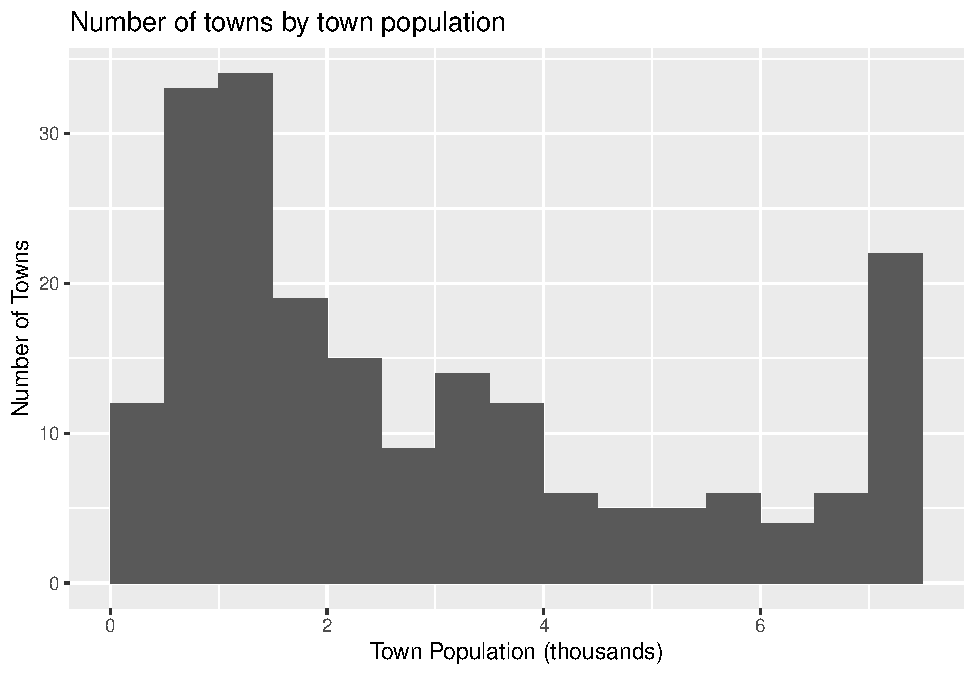
\includegraphics[width=0.7\linewidth]{IO2_PS2_Estrada_files/figure-latex/figure2-1} \end{center}

\subsection{Table 3}\label{table-3}

\begin{Shaded}
\begin{Highlighting}[]
\KeywordTok{datasummary_skim}\NormalTok{(data, }\DataTypeTok{out =} \StringTok{"markdown"}\NormalTok{, }\DataTypeTok{histogram =} \NormalTok{F, }\DataTypeTok{title =} \StringTok{"Table 3"}\NormalTok{)}
\end{Highlighting}
\end{Shaded}

\begin{longtable}[c]{@{}lrrrrrrr@{}}
\caption{Table 3}\tabularnewline
\toprule
& Unique & Missing Pct. & Mean & SD & Min & Median & Max\tabularnewline
\midrule
\endfirsthead
\toprule
& Unique & Missing Pct. & Mean & SD & Min & Median & Max\tabularnewline
\midrule
\endhead
ID & 202 & 0 & 328090.8 & 143299.0 & 40013.0 & 320014.0 &
560045.0\tabularnewline
TIRE & 14 & 0 & 2.6 & 2.6 & 0.0 & 2.0 & 13.0\tabularnewline
TPOP & 195 & 0 & 3.7 & 5.4 & 0.1 & 2.1 & 45.1\tabularnewline
NGRW & 58 & 0 & -0.1 & 0.1 & -1.3 & 0.0 & 0.0\tabularnewline
PGRW & 119 & 0 & 0.5 & 1.1 & 0.0 & 0.1 & 7.2\tabularnewline
OCTY & 160 & 0 & 0.3 & 0.7 & 0.0 & 0.2 & 8.4\tabularnewline
OPOP & 178 & 0 & 0.4 & 0.7 & 0.0 & 0.1 & 5.8\tabularnewline
LANDV & 166 & 0 & 0.3 & 0.2 & 0.1 & 0.2 & 1.6\tabularnewline
ELD & 198 & 0 & 0.1 & 0.0 & 0.0 & 0.1 & 0.3\tabularnewline
FFRAC & 174 & 0 & 0.7 & 0.4 & 0.0 & 0.8 & 1.3\tabularnewline
PINC & 191 & 0 & 5.9 & 1.1 & 3.2 & 5.9 & 10.5\tabularnewline
LNHDD & 62 & 0 & 8.6 & 0.5 & 6.8 & 8.7 & 9.2\tabularnewline
\bottomrule
\end{longtable}

\subsection{Table 4}\label{table-4}

\begin{Shaded}
\begin{Highlighting}[]
\CommentTok{#s = TPOP + NRGW + PGRW + OCTY + OPOP}
\CommentTok{#V = A + FFRAC +ELD + PINC + LNHHD}
\end{Highlighting}
\end{Shaded}

\end{document}
